%%%%%%%%%%%%%%%%%%%%%%%%%%%%%%%%%%%%%%%%%%%%%%%%%%%%%%%%%%%%%%%%%%%%%%%%
%                                                                      %
%     File: Thesis_Introduction.tex                                    %
%     Tex Master: Thesis.tex                                           %
%                                                                      %
%     Author: Francisco Castro                                         %
%     Last modified : 15 Jan 2024                                       %
%                                                                      %
%%%%%%%%%%%%%%%%%%%%%%%%%%%%%%%%%%%%%%%%%%%%%%%%%%%%%%%%%%%%%%%%%%%%%%%%


\chapter{Introduction}
\label{chapter:introduction}

%	Introdução geral a exploração planetária e em particular exploração com rovers

Space robotics covers all robotic systems which operate off the Earth. Firstly, these systems may be  classified according to its operational environment, whether it is planetary or orbital. On a second stage, a space robot is comprised of locomotion and autonomy features depending on its goal \cite{Gao2017}.

Space robot locomotion may be of several types like manipulation, gripping, roving, drilling, sampling, flying, floating, diving or even climbing. On the other hand, a space robot's autonomy ranges from teleoperation to fully-autonomous operations, while other robots execute tasks on a semi-autonomous operation mode.

In 1981, the first orbital robot, Canadarm, was placed on orbital environment with the goal to move payloads from the Space Shuttle to a given deployment position \cite{roboticsHandbook_chap55}. Later in 2001, Canadarm 2 was launched in order to assist astronauts during \acrshort{eva}, but also to maintain and build the ISS. The humanoid robot Robonaut 2 was launched to the \acrshort{iss} in 2011 to gain experience while performing assisting or teleoperation tasks, for the sake of upgrading it to a future version in order to assist astronauts during \acrshort{eva}. The Moon sampler Surveyor 3 was the first planetary robot to be launched (1967). From the 90s onwards, Mars has become the main exploratory target for surface robots. The \textit{Sojourner} rover, the twin Spirit and Opportunity \acrshort{mer} and the \acrshort{msl} have provided valuable scientific information and have enabled ground teams to design rovers which reach higher velocities and larger lifetimes. Recently, in 2021, the Perseverance rover landed on Mars taking on its belly a small robotic helicopter which accomplished the first powered, controlled flight on the thin atmosphere of Mars\footnote{https://www.space.com/mars-helicopter-ingenuity-first-flight-success (accessed on 23 of March 2026)}.

Robots which operate without human intervention have a limited lifetime, which places a limit on the returned scientifical profit. This thesis will focus on providing a navigation method which aims at delivering a safe path, while going through it in a timely fashion at a known location.

%%%%%%%%%%%%%%%%%%%%%%%%%%%%%%%%%%%%%%%%%%%%%%%%%%%%%%%%%%%%%%%%%%%%%%%%
\section{Motivation}
\label{section:motivation}

A conventional planetary, autonomous rover typically assumes a 6-wheeled articulated configuration proposed by Bekker in the 60s, after comparing several designs including tracked or screw-type vehicles \cite{roboticsHandbook_chap55, Bekker1964}. This configuration fosters crossing of crevasses, rocks or steps up to three times the radius of the wheel, while generating greater stability, redundancy, continuous wheel contact with the terrain to enforce tractability and better distribution of the vehicle load \cite{Thoesen2021}.

%Although this thesis will not focus on robot design, but rather on delivering a proposal for its \acrshort{gnc} system, it is worth mentioning alternative configurations.  Additional \acrshort{dof} and active suspensions on a 6-wheeled configuration (for instance the rocker-bogie system \citep{heverty:rockerBogie, nayar:rockieBogieDesign}) to counteract obstacles in an energy-efficient manner, is an example extensively discussed in the literature. Screw-type vehicles \cite{thoesen:spv} like helical geometries and blades are a useful configuration to generate thrust on unconsolidated or amphibious environments, where wheels cannot react against the terrain in order to generate thrust. Alternative configurations like climbing robots have been on experimental stage for space as well. The use of microspines \cite{shiquan:microspine} by reacting to passive pulling away from a non-horizontal surface is a recent development on climbing robots research. Repelling robots which rely on a tether as an anchor is a proposed method as a way to perform subsurface exploration \cite{manterola:axelRover}.

As it is stated in Table \ref{tab:roverAchievements}, launched planetary, autonomous rovers have achieved higher lifetimes as well as higher traverse speeds and travelled greater distances each mission goes by. Below, only rovers deployed in Mars are shown, but the CNSA has also deployed two rovers on the Moon, - \textit{Yutu and Yutu-2} - of which little information is known.

\begin{table}[!htb]
	\caption{Planetary, autonomous, wheeled rovers achievements.}
 	\label{tab:roverAchievements}
  	\footnotesize
  	\setlength{\tabcolsep}{5pt}
  	\renewcommand{\arraystretch}{1.2} % more space between rows
  	\centering
  	\begin{threeparttable}
  		\begin{tabular}{lcccc}
			\toprule
        	\textbf{Rover} & \textbf{Mass (kg)} & \textbf{Lifetime (sol)} & \textbf{Distance travelled (km)} & \textbf{Max. traverse speed (cm/s)}\\
        	\midrule
        	\textit{Sojourner} \cite{Gao2017, Heverly2013} & 10 & 83 & 0.106 & 0.6 \\
        	Spirit \cite{Gao2017, Heverly2013} & 185 & 2623 & 7.73 & 1.0\\
        	Opportunity \cite{Gao2017, Heverly2013} & 185 & 5352 & 45.16 & 1.0\\
        	Curiosity \cite{Gao2017, Heverly2013} & 899 & 4068 & 31.15 & 2.5\\
        	Perseverance \tnote{1, 2} & 1025 & 1021 & 23.776 & 4.2\\
        	\textit{Zhurong} \tnote{3, 4} & 240 & 347 & 1.921 & n.a.\\
        	\bottomrule
      	\end{tabular}
 		\begin{tablenotes}
			\footnotesize
			\item[1] \url{https://science.nasa.gov/mission/mars-2020-perseverance/} (accessed on 23 March of 2026)
			\item[2] Still in operation (as of March 2026)
			\item[3] Inactive
			\item[4] \url{https://en.wikipedia.org/wiki/Zhurong_(rover)} (accessed on 23 March of 2026)
		\end{tablenotes}
	\end{threeparttable}
\end{table}

Although deployed rovers have achieved greater coverages, these have also faced slippage-hazardous situations \cite{Gonzalez2017} and are subject to get around uncrossable obstacles or stay away from wind devils. These may damage the rover systems, cause progress delay or determine the end of the mission.

Slippage-related hazards play an important role on preventing a rover to achieve its proposed goals. Even though some slip is desirable to generate traction, excessive slip will result in loss of traction \cite{Wong2001} and possibly entrap the rover. These events are directly linked to the type of wheel-soil interaction taking place \cite{Genta2012}. The nature of this interaction takes into account both the type of wheel (rigid or compliable) and its features as well as the type of soil (firm or deformable) and its properties. Apart from it, other variables weighing into slip are the vertical load acting on the soil by the wheel and sinkage, which will cause a decrease on effective thrust and decrease drawbar pull \cite{wong:terramechanics, wong:performance}. In this thesis, \textbf{only rigid wheels are used}. These face higher slips on deformable ground, due to high sinkage and shear displacement, while slip is tremendously reduced in the case of compact soils \cite{Green1971}. Due to the impossibility of mimicing deformable ground dynamics on real-time simulation test-bed, only rigid terrains are considered. In Table \ref{tab:roverHazards}, one can find slippage events faced by wheeled, autonomous rovers in planetary environment as well as the teleoperating actions put in place to attempt a reversal from the state the rover was at.

\begin{table}[!htb]
	\caption[Slippage-related hazards faced by rovers at planetary environments.]{Slippage-related hazards faced by rovers at planetary environments \cite{Gonzalez2017}.}
  	\label{tab:roverHazards}
  	\footnotesize
  	\setlength{\tabcolsep}{0.5pt}
  	\renewcommand{\arraystretch}{1.5} % more space between rows
  	%\centering
      \begin{tabular}{lcccc}
        \toprule
        \textbf{Rover} & \textbf{Date of Event} & \textbf{Terrain, Place} & \textbf{Hazard} & \textbf{Action} \\
        \midrule
        Curiosity & May 2015 & \multicolumn{1}{p{4.2cm}}{\centering {\fontsize{7}{6}\selectfont Deformable terrain (Mars,\\Gale Crater, nearMount Sharp)}} & \multicolumn{1}{p{4.2cm}}{\centering {\fontsize{8}{6}\selectfont High-slip events}} & \multicolumn{1}{p{4cm}}{\centering {\fontsize{7}{6}\selectfont Turn back the rover before it\\could become entrapped}}\\
        %%%
        Curiosity & Feb 2014 &  \multicolumn{1}{p{4.2cm}}{\centering {\fontsize{7}{6}\selectfont Deformable terrain (Mars, Gale\\Crater, nearMount Sharp)}} & \multicolumn{1}{p{4.2cm}}{\centering {\fontsize{7}{6}\selectfont High-slip events (sinkage up to\\0.15 [m] and slippage up to 77\%)}} & \multicolumn{1}{p{4cm}}{\centering {\fontsize{7}{6}\selectfont The route was manually biased\\to avoid soft sands}}\\
        %%%
        Opportunity & Apr 2010 & \multicolumn{1}{p{4.2cm}}{\centering {\fontsize{7}{6}\selectfont High windblown ripple dominated\\by loose, poorly sorted basaltic\\sands (Mars, Meridiani Planum)}} & \multicolumn{1}{p{4.2cm}}{\centering {\fontsize{7}{6}\selectfont Opportunity experienced\\
significant slippage (up to 40\%)}} & \multicolumn{1}{p{4cm}}{\centering {\fontsize{7}{6}\selectfont More power to the\\wheels and extra slip checks}}\\
        %%%
        Spirit & May 2009 & \multicolumn{1}{p{4.2cm}}{\centering {\fontsize{7}{6}\selectfont Soft soil (Mars, Gusev\\Crater, Home Plate)}} & \multicolumn{1}{p{4.2cm}}{\centering {\fontsize{7}{6}\selectfont Spirit got entrapped with no\\possibility of recovery}} & \multicolumn{1}{p{4cm}}{\centering {\fontsize{7}{6}\selectfont Several recovery techniques\\(mission concluded on\\May 24, 2011)}} \\
        %%%
        Opportunity & Apr 2005 & \multicolumn{1}{p{4.2cm}}{\centering {\fontsize{7}{6}\selectfont Sand dune (Mars, Purgatory\\Ripple, Meridiani Planum)}} & \multicolumn{1}{p{4.2cm}}{\centering {\fontsize{7}{6}\selectfont Opportunity got entrapped}} & \multicolumn{1}{p{4cm}}{\centering {\fontsize{7}{6}\selectfont Recovery actions (for 5 weeks)}}\\
        %%%
        Sojourner & Aug 1997 & \multicolumn{1}{p{4.2cm}}{\centering {\fontsize{7}{6}\selectfont Deformable terrain (Mars,\\Ares Vallis)}} & \multicolumn{1}{p{4.2cm}}{\centering {\fontsize{7}{6}\selectfont The right front wheel was parked\\on a small rock, perching the left\\front wheel above the surface}} & \multicolumn{1}{p{4cm}}{\centering {\fontsize{7}{6}\selectfont Engineers teleoperated the\\rover to a safer place}} \\
        \bottomrule
      \end{tabular}
\end{table}

Very small velocities have been achieved by planetary rovers until this point. Apart from lunar teleoperated/driving vehicles, wheeled, autonomous robots have not experienced a dynamic terramechanics regime. In \cite{rodriguezHighSpeedRoversReview}, a technical review on strategies to increase the operational velocity is presented. In this thesis, a wheeled, autonomous robot is considered to be on high-speed, if it approaches or surpasses 1 m/s, which is roughly one hundred times larger than the maximum traverse rover velocities presented in Table \ref{tab:roverAchievements}.

%The Bekker method \cite{bekker:terra1956, bekker:terra1960, bekker:terra1969} is capable of providing a definition of the stress fields developed as a result of the interaction between the terrain and the vehicle wheels. However, this method is only accurate on a quasistatic regime, as it fails to accurately quantify soil behaviour in a dynamic regime. Pope stated that the rate of penetration plays a role on determining the normal stress distribution applied on the wheel \cite{pope:dynamicTerra}. Therefore, not only the slip ratio but also the vehicle's absolute speed is a factor, when it comes to determining both its sinkage and rolling resistance  under an irregular terrain. In 1971, Pope proved that by increasing the vehicle velocity, it is also possible to reduce rolling resistance and its sinkage \cite{pope:velocity}. In 1991, Grahn proposed a model which takes the Bekker pressure-sinkage relationship as its basis, but extends the formulation to include a dynamic regime (considered by Grahn to happen above 1 cm/s), by relating the rate of penetration of a rigid wheel with the wheel driving speed and slip ratio \cite{grahn:dynamicTerra}. From Grahn's model, it can be inferred that, for a given load, the maximum sinkage decreases with increasing traveling velocities. Additional details on the mentioned models and empirical evidence from planetary missions which involved high-speed vehicles can be found in \cite{rodriguez:highSpeed}.

\textbf{Slippage compensation strategies} \cite{Gonzalez2017} shall be included as a safety layer of a navigation control architecture in order to avoid entrapment or embedding situations. These solutions range from torque-based compensation solutions to velocity-based solutions. \textbf{Torque-based solutions} include maximizing traction while ensuring the soil never fails or limiting the torque control signal such that the desired slip matches the estimated slip. These methods - also called motor-current slippage compensation methods - rely on complex terramechanics models, which require the measure of several parameters in real-time, thus limiting the robot's velocity. Conversely, \textbf{velocity-based slippage compensation methods} do not require estimation of parameters from terramechanics models, though these are expected not to perform well in challenging terrain like slopes or sand ripples. This latter approach may include solutions which aim at resolving the so-called kinematic incompatibility problem \cite{Gonzalez2019} - "wheel fighting" as a result of wheel slip on irregular, off-the-road terrains -, adapt control signals with respect to the estimated slip and limit the velocity and acceleration of wheels, although this latter approach may result in non-controllable slip hazards because the robot will slip even with a limited motion domain.

%%%%%%%%%%%%%%%%%%%%%%%%%%%%%%%%%%%%%%%%%%%%%%%%%%%%%%%%%%%%%%%%%%%%%%%%
\section{Problem Statement}
\label{section:problemStatement}

As a result of tackling these issues, this thesis will focus on developing an optimal control method that aims to \textbf{maximize the operational timeline}, by decreasing the time dedicated to go through the planetary environment to reach locations of scientific interest and increase the available time for scientific operations. Extending the covered surface is also a desirable navigational outcome, which may be eased by providing the robot with a prior knowledge of the scouting area \cite{Coombs2000, Urmson2004}. Therefore, this thesis will focus on providing a navigational control architecture which addresses the issues presented previously, by taking \textbf{safety, fastness and covered area as the main metrics of success}.

Apart from that, the control architecture shall capture the dynamics of the mobile robot and be able to cope with rough, uneven terrain. Moreover, the safety of the robot shall not be safeguarded only by the control module, but also by yielding a global path that ensures these metrics of sucess are more easily achieved.

\section{Project outline}
\label{section:projectOutline}

First, the definition of the mobile robot dynamics comes as the first challenge to address. This problem shall take into account the mobile robot geometric features as well as the environment the wheeled mobile robot will be moving on.

\begin{figure}[!h]
	\centering
	\tikzstyle{block} = [draw, text centered, minimum height = 2.0em,minimum width = 7.5em, rounded corners, line width = 0.5 mm]
	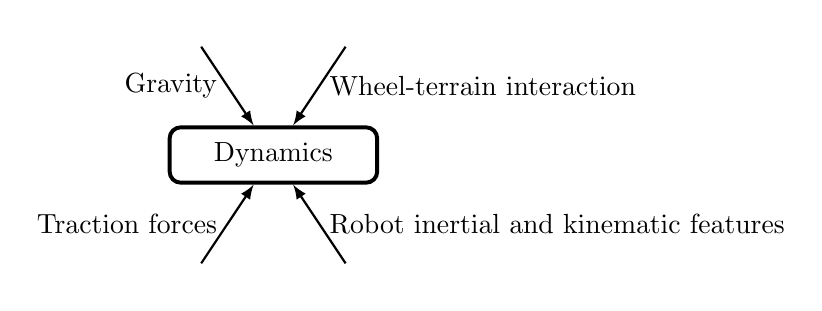
\begin{tikzpicture}
		\node [block, align = center] at (4.5, 0) (3) {Dynamics};
		\node at (3.5, 1.5) (6) {};
		\node at (3.5, -1.5) (7) {};
		\node at (5.5, 1.5) (8) {};
		\node at (5.5, -1.5) (9) {};

  		\draw [-latex,thick] (6) --  node [left] {Gravity} (3);
  		\draw [-latex,thick] (7) --  node [left] {Traction forces} (3);
  		\draw [-latex,thick] (8) --  node [right] {Wheel-terrain interaction} (3);
  		\draw [-latex,thick] (9) --  node [right] {Robot inertial and kinematic features} (3);
	\end{tikzpicture}
	\caption{Outline of mobile robot dynamics.}
    \label{fig:outlinerobotdynamics}
\end{figure}

Then, the generation of a safe and fast path comes as the next problem to face. From the elevation map of the terrain, a cost map shall be generated, that expresses the adaptation of the mobile robot to the terrain, by taking into the terrain uneveness and the vehicle hull. From there, it may be possible to extract a path from the traversability map.

\begin{figure}[!h]
	\centering
	\tikzstyle{block} = [draw, text centered, minimum height = 2.0em,minimum width = 7.5em, rounded corners, line width = 0.5 mm]
	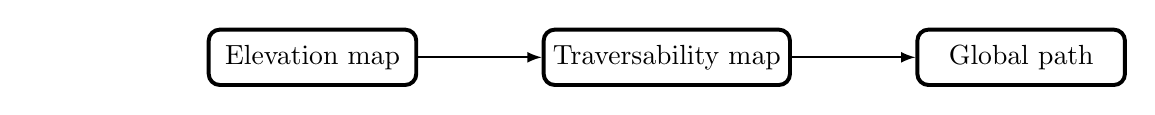
\begin{tikzpicture}
		\node at (-3.5, 0.0) (1) {};
		\node [block, align= center] at (0, 0) (2) {Elevation map};
		\node [block, align = center] at (4.5, 0) (3) {Traversability map};
		\node [block, align = center] at (9.0, 0) (4) {Global path};
		
  		\draw [-latex,thick] (2) --  node [above] {} (3);
  		\draw [-latex,thick] (3) --  node [above] {} (4);
	\end{tikzpicture}
	
	\caption{Generation of global path outline.}
    \label{fig:outlineglobalpathgen}
\end{figure}

Finally, a controller that is aware of the mobile robot dynamics and the reference to track comes to mind as the way to provide proper guidance under this extreme scenario. The controller shall also avoid collisions and redirect the path if needed. This control module is the main focus of the thesis, as it is the system that mainly guarantees the vehicles's safety and fastness along the traversal.

\begin{figure}[!h]
	\centering
	\tikzstyle{block} = [draw, text centered, minimum height = 2.0em,minimum width = 7.5em, rounded corners, line width = 0.5 mm]
	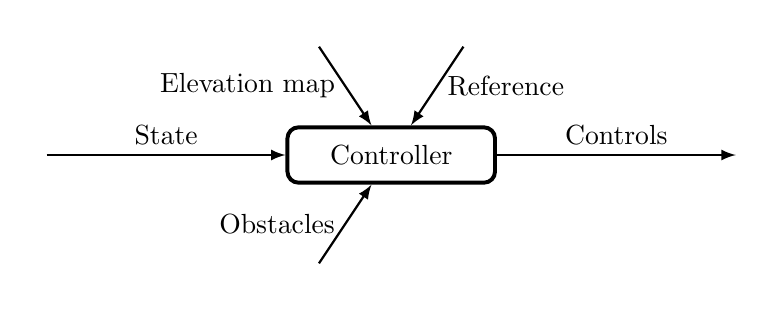
\begin{tikzpicture}
		\node [align= center] at (0, 0) (2) {};
		\node [block, align = center] at (4.5, 0) (3) {Controller};
		\node [align = center] at (9.0, 0) (4) {};
		\node at (3.5, 1.5) (6) {};
		\node at (3.5, -1.5) (7) {};
		\node at (5.5, 1.5) (8) {};
		\node at (5.5, -1.5) (9) {};
		
  		\draw [-latex,thick] (2) --  node [above] {State} (3);
  		\draw [-latex,thick] (3) --  node [above] {Controls} (4);
  		\draw [-latex,thick] (6) --  node [left] {Elevation map} (3);
  		\draw [-latex,thick] (7) --  node [left] {Obstacles} (3);
  		\draw [-latex,thick] (8) --  node [right] {Reference} (3);
	\end{tikzpicture}
	
	\caption{Input-output plot of controller.}
    \label{fig:controlleroutline}
\end{figure}

%%%%%%%%%%%%%%%%%%%%%%%%%%%%%%%%%%%%%%%%%%%%%%%%%%%%%%%%%%%%%%%%%%%%%%%%
\section{Objectives}
\label{section:objectives}

In order to achieve a reasonable implementation of the project outline, but also to effectively meet the demands of the problem description, the following goals are stated:

\begin{enumerate}
\item \textbf{Dynamics identification}
	\begin{enumerate}
		\item Selection of a four-wheeled rigid mobile robot and retrieve its inertial and geometric features;
		\item Selection of a wheel-terrain interaction regime that one may properly simulate;
		\item Identification of all external forces acting on the robot;
		\item Model validation.
	\end{enumerate}
\item \textbf{Global path plan generation}
	\begin{enumerate}
		\item Selection of elevation map to work on top of;
		\item Generation of traversability map that expresses the difficulty to traverse each point of the map, with respect to the selected mobile robot hull;
		\item Global path generation that avoids untraversable positions and enables a fast overall traversal of the map.
	\end{enumerate}
\item \textbf{Development of an optimal control algorithm that copes with extreme terrain}
	\begin{enumerate}
		\item Survey and selection of optimal control architectures;
		\item Tuning of the controller parameters;
		\item Path tracking capability verification;
		\item Augmentation of the controller to enable collision avoidance;	
		\item Real-time feasibility verification;
	\end{enumerate}
\end{enumerate}


\section{Contributions}
\label{section:contributions}

Along the work presented in this thesis, the following contributions were achieved:

\begin{enumerate}
	\item Revisitation of \cite{Amorim2014} and development of a \textbf{worst-case traversability map that considers the terrain roughness and inclination}. On top of it, the traversability map is refined to penalize positions bordering highly untraversable areas. In \cite{Amorim2014}, only the terrain inclination is considered.
	\item Extensive testing of a real-time \acrlong{nmpc} path-tracking algorithm is also delivered. The algorithm copes well with rough terrain and prevents slippage.
	\item Development of a novel \textbf{safe real-time path-tracking \acrlong{nmpc} algorithm}. This algorithm sucessfully prevents the mobile robot from entering unsafe areas of the map. The closest implementation of a similar algorithm that was found in the literature was performed in smooth terrain and did not respect real-time requirements \cite{yu2022nmpc}. Some real-time control applications to rough terrain were found, but these were solely performed along the longitudinal direction \cite{IagnemmaDubowsy2004, rathod2021model}.
\end{enumerate}

%%%%%%%%%%%%%%%%%%%%%%%%%%%%%%%%%%%%%%%%%%%%%%%%%%%%%%%%%%%%%%%%%%%%%%%%
\section{Thesis Outline}
\label{section:outline}

This thesis is structured as follows:

\begin{itemize}
\item \textbf{Chapter 2}: The literature related to each of the subjects mentioned in section \ref{section:objectives} is laid out.
\item \textbf{Chapter 3}: The dynamics identification and validation of the mobile robot is performed here. Moreover, several steering mechanics are also compared as well cost function formulations of the \acrlong{ocp} that will accomodate the dynamics model.
\item \textbf{Chapter 4}: The theoretical background that is behind the development of a global path planner and the optimal control algorithm is presented.
\item \textbf{Chapter 5}: The implementation of first contribution of this thesis is detailed. The fast marching method was chosen so that a global optimal potential field properly guides the path generation without falling into local minimums.
\item \textbf{Chapter 6}: The implementation of the second contribution of this thesis is presented here.
\item \textbf{Chapter 7}: The implementation of the last contribution of this thesis is laid out here.
\item \textbf{Chapter 8}: This chapter reviews the whole work and points to its deficiencies. Some research directions that may be followed on top of this thesis are also proposed.
\end{itemize}